\documentclass[12pt, oneside]{article} 
\usepackage{booktabs}
\usepackage{geometry}              	
\usepackage{adjustbox}
\usepackage{pdfpages}  		
\usepackage{graphicx}
\usepackage{caption}						
\usepackage{amssymb}
\usepackage{amsmath}
\usepackage{pdfpages} 
\usepackage{longtable}
\usepackage{subfig}
\usepackage{url}
\usepackage{comment}

%\usepackage{subcaption}
\usepackage{graphicx}  % remove 'demo' option for your real document

\usepackage{fancyvrb}
\usepackage{hyperref}
\usepackage{titlesec}
\usepackage{fancyhdr}
\usepackage{blindtext}
\usepackage{graphicx}
\usepackage{longtable}
\usepackage{booktabs}
\usepackage{multirow}
%\usepackage[dvipsnames]{xcolor}
\usepackage{pdflscape}
\usepackage{subfig}
\setcounter{tocdepth}{6}
\setcounter{secnumdepth}{6}
\titleformat{\paragraph}
{\normalfont\normalsize\bfseries}{\theparagraph}{1em}{}

 \setlength{\headheight}{14.5pt}
\lhead{}
 
\usepackage[english]{babel}
\usepackage[utf8]{inputenc}

\geometry{left=2.0cm,right=2.0cm,top=2.0cm,bottom=2.0cm}
%using the euro symbol
\usepackage[utf8]{inputenc}
\usepackage{marvosym}
\DeclareUnicodeCharacter{20AC}{\EUR{}}
%\usepackage[dvipsnames]{xcolor}
\usepackage{array,tabularx,calc}
%to allow use of < and >
\usepackage[T1]{fontenc}
%references
\usepackage{csquotes}
%\usepackage[style=nature]{biblatex}
%\addbibresource{references.bib}
\newlength{\conditionwd}
\newenvironment{conditions}[1][where:]
  {%
   #1\tabularx{\textwidth-\widthof{#1}}[t]{
     >{$}l<{$} @{${}={}$} X@{}
   }%
  }
  {\endtabularx\\[\belowdisplayskip]}

\usepackage{array,tabularx}

\newcommand{\HRule}[1]{\rule{\linewidth}{#1}} 	% Horizontal rule

\makeatletter							% Title
\def\printtitle{%						
    {\centering \@title\par}}
\makeatother
									

\makeatletter							% Author
\def\printauthor{%					
    {\centering \large \@author}}				
\makeatother	

\usepackage{mathtools} 

\usepackage[font=small,labelfont=bf]{caption}

\begin{document}


\begin{titlepage}
	\centering 
	\scshape
	\vspace*{2\baselineskip}
	\rule{\textwidth}{1.6pt}\vspace*{-\baselineskip}\vspace*{2pt} 
	\rule{\textwidth}{0.4pt} 
	%\vspace{0.75\baselineskip} 
	%{\Huge PHYC40600 \\ Advanced Physics Lab II} \\
	\vspace{0.1in}
		{\Large Ruth Moore } \\
		\vspace{0.1in}
		{\Large Supervisor - Dr Anaïs Orsi} \\
	\vspace{0.75\baselineskip} 
	\rule{\textwidth}{0.4pt}\vspace*{-\baselineskip}\vspace*{2pt} 
		\rule{\textwidth}{1.6pt}
	\vspace*{2\baselineskip} 

\Huge{Polar Amplification in the Western Canadian Arctic}
\vspace{0.1in}	

\begin{figure}[hbtp]
\centering

\includegraphics[width=0.5\textwidth]{figures/ubc-logo-png-transparent.png}
\end{figure}
{\Large September 2021- } \\
	{\large University of British Columbia} 
\end{titlepage}
\pagestyle{fancy}
\tableofcontents
\thispagestyle{empty}
\clearpage
\setcounter{page}{1}


\pagebreak
\begin{abstract}


\end{abstract}

{\color{blue}note: blue text is writing notes which will be deleted and ?? denotes areas where information has to be added 

\subsection{Goal of the introduction}
To organise learning in a detailed way 
What is the question that I am looking at?
Show all of the information that is known 
Why and how do we know this - why is this interesting and relevant to this project?
What is the framework for how we compare and contrast ideas?
Why this study is doable}
\section{Introduction}
{\color{blue}
- The Arctic in the global climate system
- explain how the complexity of the environment is different in different regions (comparing the Russian Arctic to Canadian etc based on geography).
}

Considerable progress has been made in the understanding of polar amplification in the Arctic over the last decades, the phenomenon in which the poles are warming more quickly than the rest of the world. In recent
years we have begun to understand why these changes are
occurring, and increasingly the cause for this warming has been attributed to an increase in
precipitation and humidity. Considerable work has been done in various areas of the Arctic with few studies focusing on the Western Canadian Arctic (WCA). 

Since these changes rely heavily on local geography and weather, more work needs to be done in investigating these changes in the WCA. This project aims to investigate the dominant changes in atmospheric humidity overtime in the WCA, to help gain a better understanding of changes in the region. 

\subsection{The Arctic within the global climate system}
The Arctic is closely linked to the rest of the global climate system. The loss of the Greenland Ice Sheet and other Arctic land contribute more to the global sea level rise than then melting of Antarctica \cite{amap}. Wildfires result in carbon emission to the atmosphere. Changes effect local livlihoods, migrating animals and economic activities such as shipping routes and mining. 
%Changes in the climate of the Arctic have a strong effect on 

\subsubsection{Characterising change}
Arctic climate change is mainly characterised by a warmer and wetter atmosphere due to the overall global increase in temperature. Polar amplification is causing these changes, which is driven by the mechanism of poleward energy transport, the snow and ice albedo feedback and water-vapour radiative feedbacks. 

%In accordance 
\subsection{Polar amplification}\label{polar_amplification}
{\color{blue}{How this effects 
- seasons
- sea ice changes }}

Polar amplification is the phenomenon in which any net change in radiation balance on Earth, such as a the greenhouse effect produces larger temperature changes near the poles than the rest of the planet. Three main processes are driving this amplification, the loss of sea ice and snow, the confinement of warming to the near surface in the polar atmosphere and the increases in poleward atmospheric and oceanic heat transport.   These are combined effects which differ between the hemispheres.

There has been a considerable loss in sea ice extent since 1979, with a yearly decrease in sea ice expected to continue with the increase in $CO_2$ in the atmosphere. With warming temperatures ice has less time to form which makes it thinner and causing it to melt earlier. 
%\subsubsection{Loss of sea ice}

%\subsubsection{Confinement of warming to the near surface}
%\subsubsection{Increase in poleward heat transport}
There has been an increase in atmospheric and ocean heat transport to the poles due to changes in the transport of latent energy (moisture) and dry static energy (the sum of sensible and potential energy) by atmospheric circulations. 

This process can be described using an Earth System Model, where eddies dominate heat transfer from the mid latitudes to the poles. As the mid latitudes warm this increase the difference in moisture between the poles and the mid latitudes causes an increase in poleward latent heat energy transport. 

This episodic increase in latent heat transport into the Arctic results in an enhancement of the surface downwelling radiation, which drives sea ice losses on sub-seasonal timescales. 

The increase in Arctic annual mean surface temperature (land and
ocean) between 1971 and 2019 was three times
higher than the increase in the global average
during the same period \cite{amap}. 
\subsubsection{Clausius-Clapeyron relation}\label{cc}
The capacity of air to hold moisture increases exponentially with air temperature according to the Clausius-Clapeyron equation. Saturated water pressure P and temperature T are related as follows;

\begin{equation}
    P \propto exp\frac{-\Delta H_{vap}}{RT}
\end{equation}
where $\Delta H_{vap}$  is the Enthalpy (heat) of Vaporization and R is the gas constant. Integrating between two pressure end points gives the Clausius-Clapeyron equation;  
\begin{equation}
    ln \left ( \frac{P_1}{P_2} \right ) = \frac{\Delta H_{vap}}{R} \left ( \frac{1}{T_2} - \frac{1}{T_1} \right )
\end{equation}

This equation allows and estimate of vapour pressure at different temperatures and visa-versa, which simplifies to an increase of water retention by around $7\% / ^{\circ} C $. This would lead to a strengthening of the global evaporation (E) minus precipitation (P) pattern with overall global surface temperature increases \cite{held2006robust}. Experimental results differ from this estimation, and it has been found to have a value closer to $3.0 \pm 1.6 \% / ^{\circ} C $ from 1950 to 2010, with climate models showing an increase of $4.3 \pm 2.0 \% / ^{\circ} C $ under greenhouse gass emission scenarios \cite{Skliris2016}. 

\subsubsection{Polar amplification in the Arctic}
Polar amplification effects the Northern Hemisphere more than the Southern Hemisphere. This is due to the larger surface heat uptake in the southern ocean and the asymmetry in radiative feedbacks in the poles. 

There is a seasonality to the phenomenon in which there is a peak of sea ice losses in early winter and increases in heat fluxes from the ocean to the atmosphere resulting in strong near surface warming. 

\subsection{Humidity}\label{humidity}

Humidity is the concentration of water vapour present in the air, and depends on the temperature and pressure of the system of interest, with three measurements used. 

\subsubsection{Relative humidity}
Relative humidity, which is the ratio of partial pressure of water vapour in a mixture (ie the air) to the equilibrium vapor pressure of water over a flat surface of pure water. This measurement is the ratio of how much water vapour is in the air versus how much it could have. 

\begin{equation}
    \phi = \frac{\rho H_O}{\rho^* H_2O}
\end{equation}

where $\rho H_O$ is the partial pressure of water vapour in the mixture and $\rho^* H_O$ is the equilibrium vapour pressure of water over a flat surface of pure water. 


\subsubsection{Relative humidity}
Absolute humidity is the mass of of water vapour per unit volume of moist air or as mass of water vapour per mass of dry air, and does not take temperature into consideration.

\begin{equation}
    AH = \frac{mH_2O}{V_{net}}
\end{equation}
Where $mH_2O$ is the mass of water vapour and $V_{net}$ is the volume of air and water vapour mixture. 

\subsubsection{Specific humidity}
Specific humidity is the ratio of water vapour mass to total moist air parcel mass. It is approximately equal to the mixing ration which is  the ration of mass of water vapour in an air parcel to the mass of dry air for the same sized parcel. 

%\subsection{Atmosphere structure}

%The atmosphere is composed of
\subsection{Hydrological cycle}
{\color{blue}- Why the moisture component is very important 
- Sources of moisture and possible changes to this }
%\subsubsection{Phenomenon which effect humidity}
{\color{blue}-  how the circulation of wind in the Arctic effects humidity 
- sea ice 
- evapotranspiration }

The hydrological cycle describes the sum total of all processes in which water moves from the land to the ocean surface to the atmosphere and back to the land/ocean in the form of precipitation \cite{CHAKRAVARTY2019203}. 

As described in section \ref{cc} an increase in global temperatures increases the overall amount of moisture in the air. Moisture content in the Arctic is closely linked to increases in moisture in the mid latitudes due to processes of poleward moisture and heat transport, as described in section \ref{polar_amplification}. The strong coupling between the mid latitude and polar hydrological cycles are thus an important component when discussing warming in the Arctic.   
{\color{blue} In summary - less snow but more rain }

\begin{figure}[h!]
\centering
\includegraphics[width=0.9\textwidth]{figures/IPCC-SROCC-CH_3_10.jpg}
\caption{Schematic of the important land surface components of the hydrological cycle influenced by the Arctic terrestrial cryosphere: permafrost (1); ground ice (2); river discharge (3); abrupt thaw (4); surface water (5); fire (6); tundra (7); shrubs (8); boreal forest (9); lake ice (10); seasonal snow (11). \cite{ipcc}}\label{fig:hydro}
\end{figure}

Figure \ref{fig:hydro} shows land surface components which contribute to the changing hydological cycle. Figure \ref{fig:hydro}.a is a time series of snow cover extent in June relative to 1981-2010 climatology from 5 models based on . Figure \ref{fig:hydro}.b shows the change in permafrost temperature normalised to a baseline period. Increasing permafrost temperatures result in ground instability, increased water run off and an overall increase in precipitation. Region A: Continuous to discontinuous permafrost in Scandanavia, Svalbard, and Russia/Siberia, Region B: Cold continuous permafrost in northern Alaska, Northwest Territories, and NE Siberia, Region C: Cold continuous permafrost in Eastern and High Arctic Canada, Region D: Discontinuous permafrost in Interior Alaska and Northwest Canada. Figure \ref{fig:hydro}.c shows annual runoff normalised to the 1981-2010 baseline ($\pm 1$ standard deviation. Figures \ref{fig:hydro}.d,e \& f are the Coupled Model Intercomparison Project Phase 5 (CMIP5) multi-model average (± 1 standard deviation) projections for different Representative Concentration Pathway (RCP) scenarios for d) June snow cover extent change, e) area change for near-surface permafrost and f) runoff change to the Arctic Ocean. 

Terrestrial, marine and freshwater ecosystems are strongly coupled with the cryosphere and atmosphere to form the Arctic hydrological cycle, as shown in fig.\ref{fig:hydro_cycle}.  


\begin{figure}[h!]
\centering
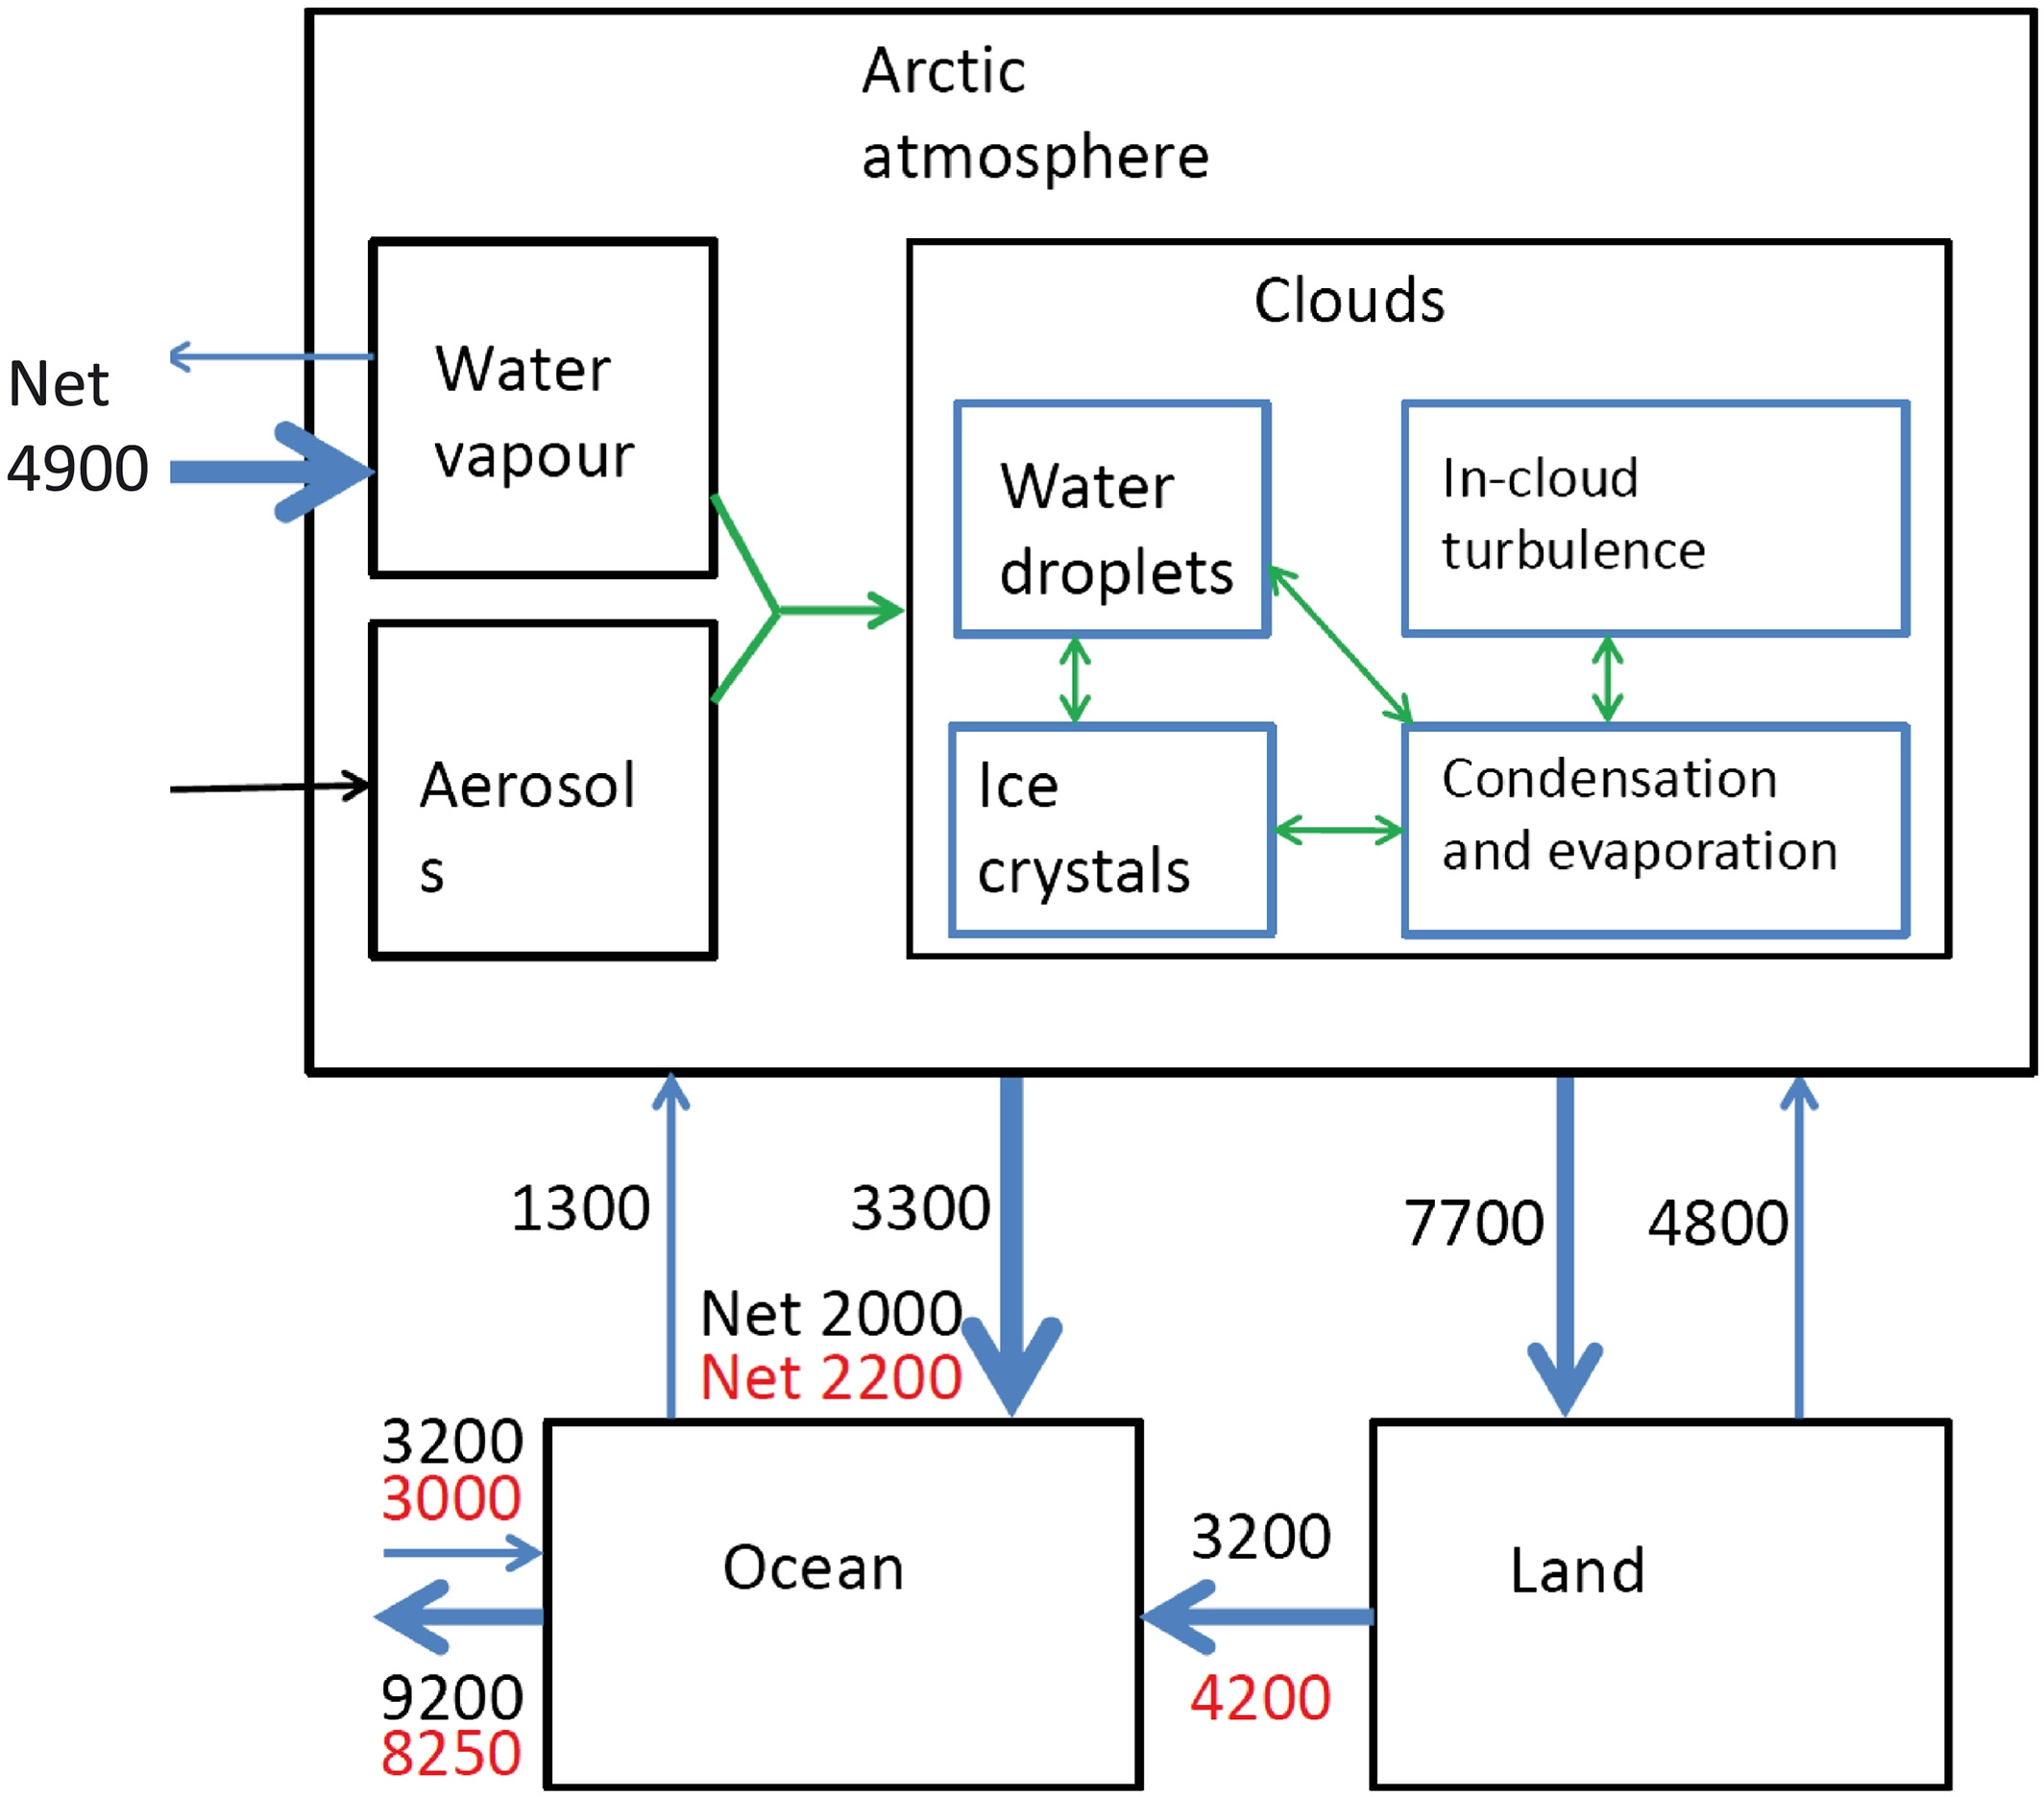
\includegraphics[width=0.7\textwidth]{figures/hydological_cycle.png}
\caption{Schematic of the main freshwater components and processes in the Arctic hydrological cycle \cite{vihma2016atmospheric}. The numbers in black show the main freshwater transports in $km^3/yr$ based on \cite{serreze2006large} for 1979-2010, with the numbers in red show the estimates for 2000-2010 from   \cite{haine2015arctic}. }\label{fig:hydro_cycle}
\end{figure}

\newpage

\subsubsection{Atmosphere}

In the polar regions the atmospheric component of the hydrological cycle is composed of a moisture flux, where precipitation (P) and evaporation (E) converge to give a and net positive precipitation (P-E). The primary input of water into the polar regions is through atmospheric moisture transport. The P-E is generally an input of freshwater from the atmosphere to the ocean \cite{oshima2017atmospheric}. 

Water vapour in the Arctic has a residence time of around a week, compared with a decade for freshwater in the Arctic ocean, with the spatial and temporal distributions of vapour relation to air temperature distributions. As explained in section \ref{cc} the moisture holding capacity of air increases exponentially with air temperature, and therefore total vertically integrated water vapour (TWV) decreases with increase in longitude, from summer to winter and is higher over the open ocean which is warmer than the cyrosphere. As a result clouds are more common over the open ocean than ice, and sparse over the continents. The amount of cloud cover reaches a maximum in the mid latitude Arctic regions in the late summer, and a minimum during the late winter. The occurance of water vapour and clouds in the Arctic is due to local evaporation and evapotranspiration and condensation due to transport to lower latitudes. The seasonal cycles of P-E over the regions are governed by cyclone cycles where interannual variations are determines by the Arctic Oscillation. 

\begin{figure}[h!]
\centering
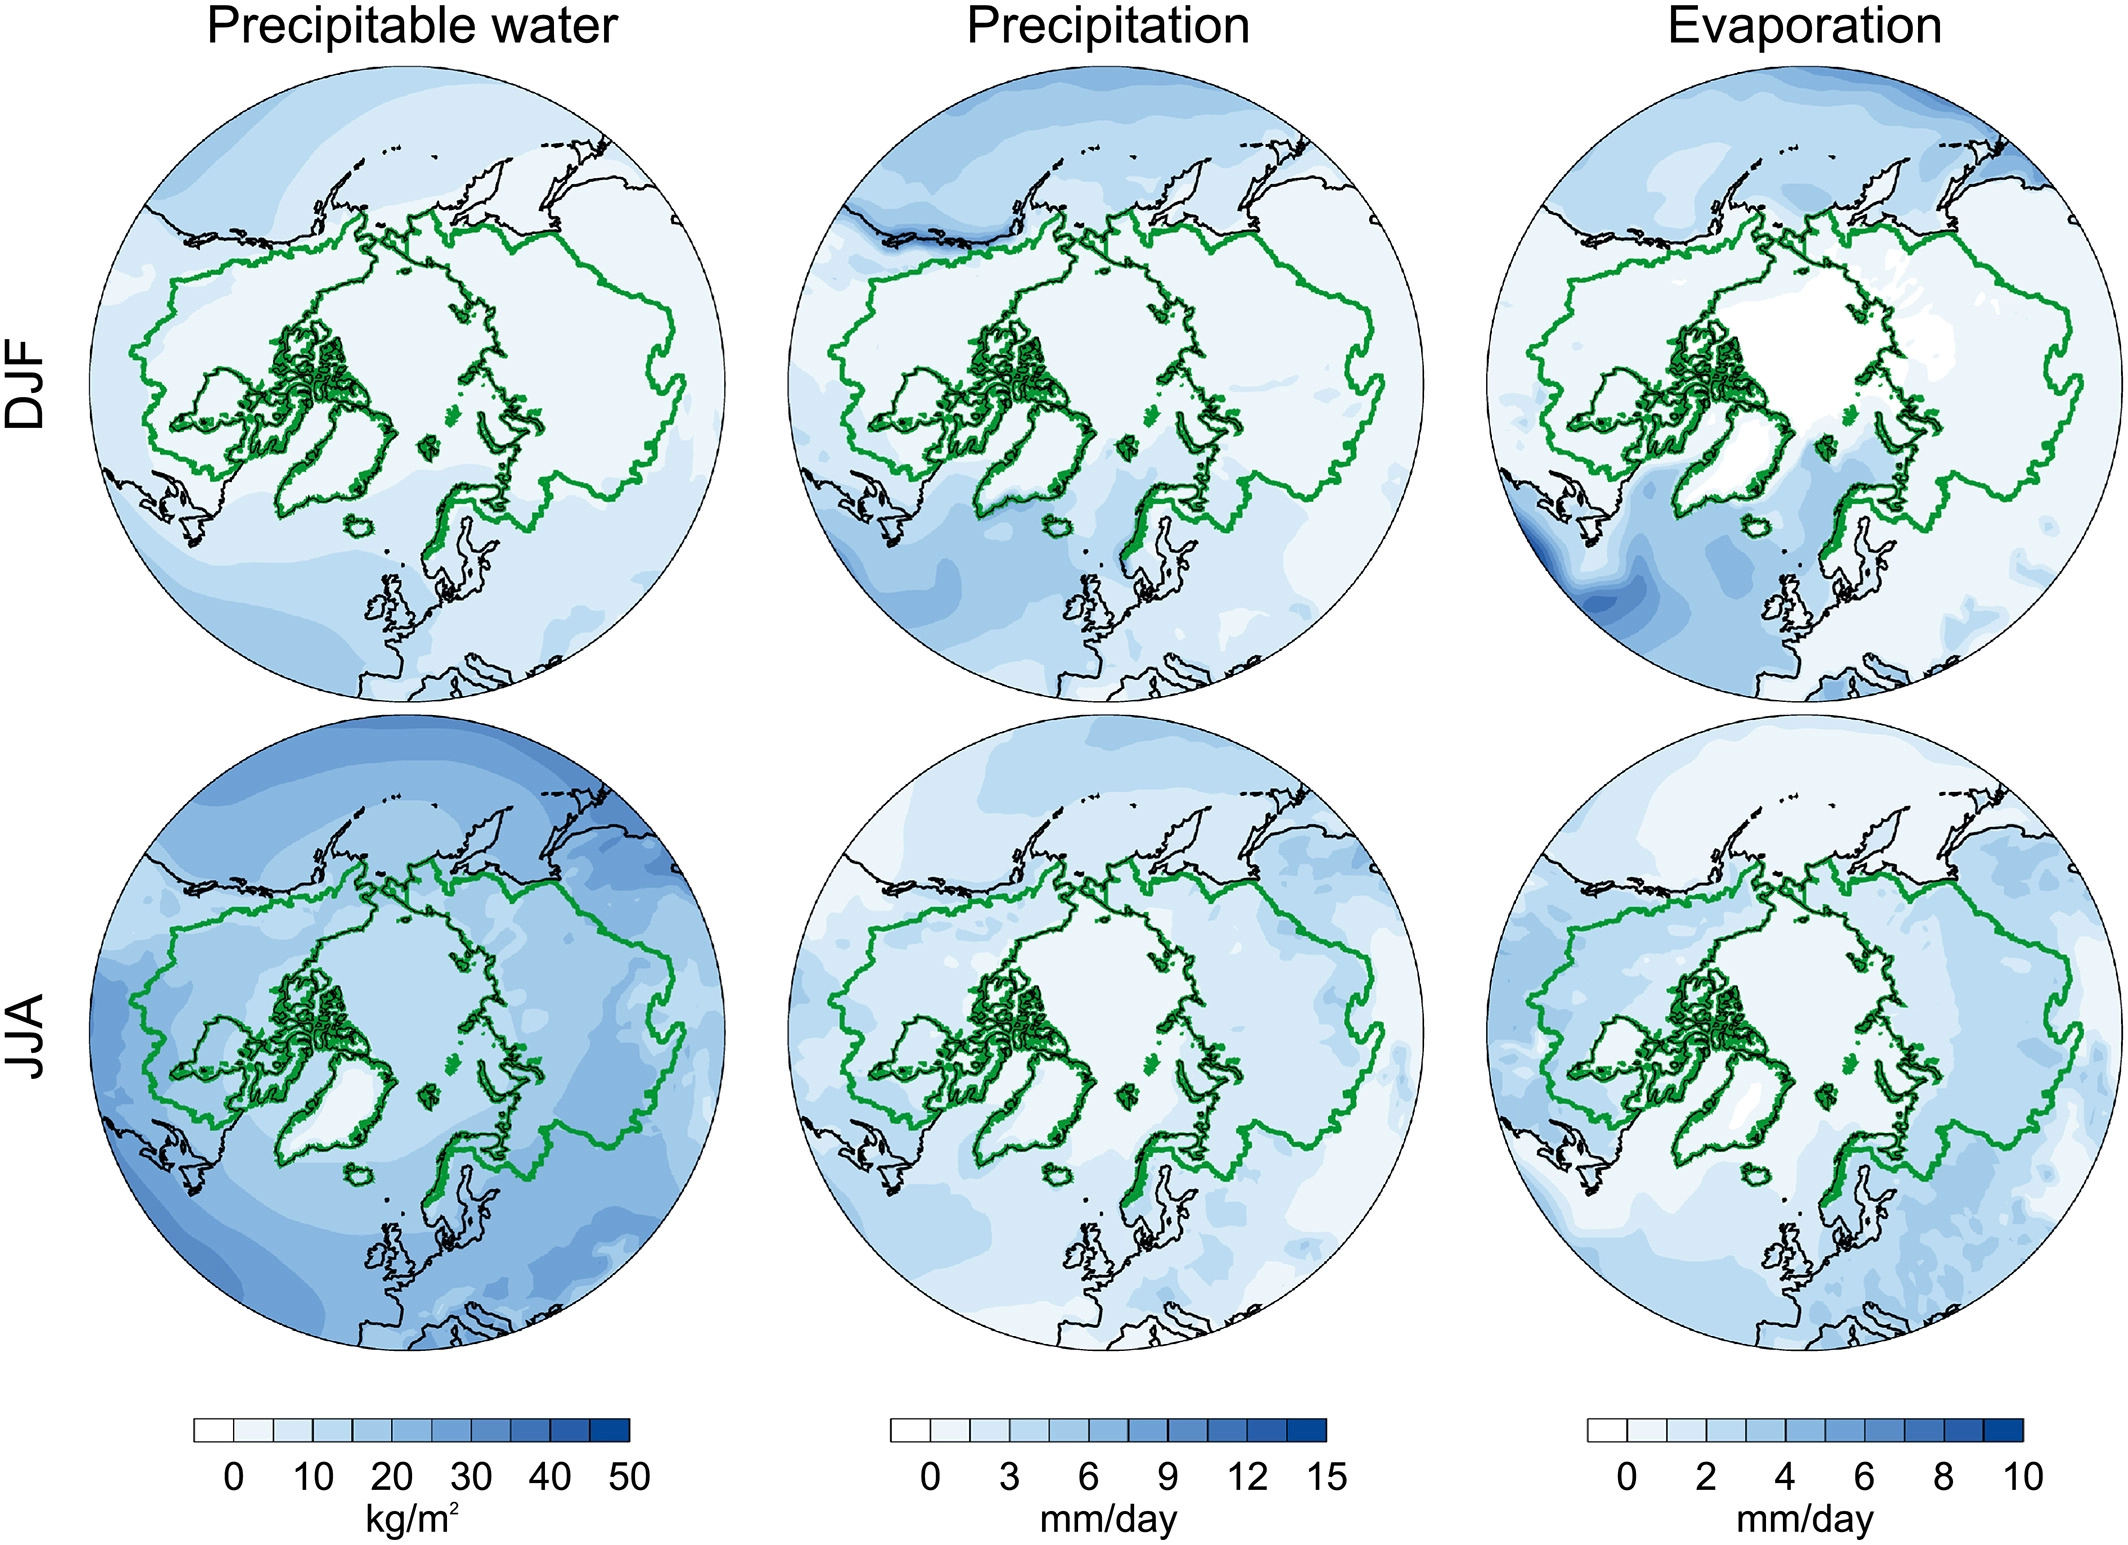
\includegraphics[width=0.7\textwidth]{figures/arctic_water_distributions.png}
\caption{Schematic of the seasonal means of preciperable water, precipitation and evaporation for winter (DJF) and summer(JJA) from 1980-2013 based on the reanalysis of the JRA-55 data set. The green lines show the bounaries of the Arctic river catchment \cite{vihma2016atmospheric}. }\label{fig:arctic_moisture}
\end{figure}

\paragraph{Atmospheric Moisture}
Atmospheric moisture is composed of water vapour which is the source of cloud and fog formation, which affect radiative transfer, evaporation and condensation, where relative humidity controls cloud formation. During cloud formation, the level where saturation is reached depends on the vertical temperature profiles and specific humidity. As the volume of unsaturated air cools, it's relative humidity increases since the ability for air to hold vapour decreases with temperature, the air temperature inversion generally occurs between 1-1.5 km but this has strong seasonal and spatial variation. 

Changes in specific humidity also effect longwave and shortwave radiative transfer in the atmosphere, where humid air emits more longwave radiation than dry air due to its humidity and temperature. 

\paragraph{Evaporation and moisture transport from lower latitudes}
The amount of moisture in the Arctic is determined by the rates of local evaporation and moisture transport from lower latitudes, see fig.\ref{fig:hydro_cycle}. Due to a large amount of evaporation from leads and polynyas, the near surface air humidity over Arctic sea ice is generally close to saturation with respect to the ice phase and therefore sublimation is weak. 

Leads are large fractures within an expanse of sea ice, where a linear area of open water is present, and often used for transport. They can vary in width from meters to hundreds of meters. Polynans are areas of open water surrounded by sea ice.

Other sources of atmospheric moisture in the Arctic is transported from lower latitudes, driven by the north-south gradient in air specific humidity and is affected by large-scale circulation patterns such as planetary waves, subtropical jet stream, the Polar front jet stream, storm track, Jalley, Ferrel and Polar cells. These phenomenon are split up into mean meridional circulation, stationary eddies and transient eddies. 

%add more detail here https://agupubs.onlinelibrary.wiley.com/doi/10.1002/2015JG003132

\paragraph{Cloud cover}
Cloud cover is difficult to determine in the Arctic due to temporal and spatial limitations, with data indicating that the Arctic has an annual cycle of cloudiness ranging from 40-70\% in winter to 80-95\% in summer. Low clouds and fog dominate and predominantly have a warming effect on the surface, especially over the ice covered part of the Arctic Ocean. Cloudy conditions are often related to a warmer free troposphere, as cloudy episodes are typically associated with advection from lower latitudes. 

\paragraph{Precipitation}
In winter the spatial distributions of precipitation and evaporation are dominated by the difference between large values over the open seas and low values over snow/ice-covered sea and land areas. In summer, both precipitation and evaporation over Arctic land areas, except Greenland, exceed the values over sea areas north of 70$^{\circ}$N and are comparable to those at lower latitudes. Precipitation and evaporation/evapotranspiration affect the ocean and terrestrial freshwater budgets, the surface albedo and energy budget, and the mass balance of ice sheets, glaciers, and sea ice. Arctic ocean freshening occurs during the snow and ice melt in the summer, with river discharge also resulting in freshening. Over continents, in most of the Arctic river catchment, net precipitation is stored as snow for half a year or more

The reduction and increase of snow cover over the seasonal cycle effects the albedo of the surface. Snow and ice surface albedo depending on several factors, such as the snow wetness, temperature, density, grain structure, impurities, melt ponds, and surface slope. 

\subsubsection{Cryosphere}
Of the components which constitute the Arctic environment, the cryosphere is the most sensitive to the effects of the changing climate \cite{rinke2019trends}. The cyrosphere, which is the ice component of the Earth's surface is closely linked with terrestrial and freshwater ecosystems, making it a crucial component within the Arctic system.

The changing cyrosphere effects the overall hydrological cycle within the Arctic, contributing to the warmer and wetter conditions which have been seen in recent years. The cryosphere amplifies climate change through snow, ice and permafrost feedbacks. 




\paragraph{Sea ice}
Sea ice amount has a natural fluctuation within the Arctic climate system throughout the year, with coverage between 5 and 6 million $km^2$ at the end of the summer to 14 million $km^2$ at the end of winter. The annual average of sea ice in the Northern Hemisphere decreased by about 7.4\% between 1978 and 2003. 

\paragraph{Snow cover}
In the Arctic, snow can account for up to 80\% of total precipitation. Snow extent and fall is crucial to the hydrological cycle, where its albedo affects surface radiation balances and water budgets and the habitat of land and water biota. Snow is an insulator affecting the thermal balances of the ground and permafrost distribution. 

Between 1972 and 2003 the average snow cover extent in the Northern Hemisphere decreased by around 10\%. The projected increases in Arctic temperature will decrease the length of time available for snow to accumulate in winter, affecting the winter snow melt, which is a major component of the hydrological cycle. 

\paragraph{Glaciers and Ice Sheets}
The majority of the total volume of ice in the Arctic is contained in Greenland, with Canada having major ice caps and glaciers in the high Arctic and Yukon. Glaciers and ice-caps across the Arctic show a general retreat among glacier fronts and overall volume decreases since the 1920s.


\paragraph{Permafrost}\label{permafrost}
The frozen component of the ground, such as rock and ice which remains permanently frozen is known as permafrost. Permafrost is composed of an upper layer which thaws during the summer and freezes again during the autumn/winter, which is known as the active layer. Permafrost covers approximately 25\% of and in the Northern Hemisphere and contains twice as much carbon as the atmosphere. 


{\color{blue}{try to find a more recent map than this one}

%https://essd.copernicus.org/articles/7/245/2015/essd-7-245-2015-metrics.html

%https://gtnp.arcticportal.org/images/Pictures/Maps/GTN-P_map_permafrostzones_Arctic.jpg
}

\begin{figure}[h!]
\centering
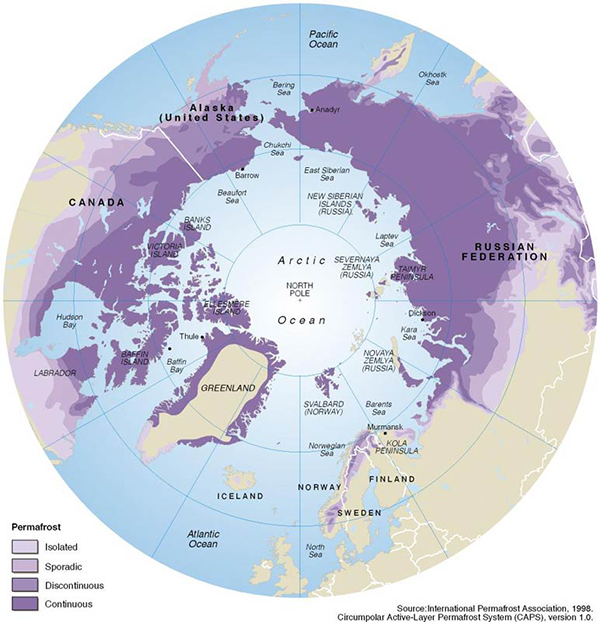
\includegraphics[width=0.6\textwidth]{figures/permafrost-arctic-distribution.png}
\caption{Map of permafrost cover, darker shades of purple indicate higher amounts of permanently frozen ground. \cite{perm_map}}\label{fig:perm}
\end{figure}



Changes in depth and extent of the active layer is an area of continuous study in relation to amplification. This has grown deeper at many sites since the 1990s and landscape observations also show considerable thaw across the Arctic. The largest magnitude of thaw is occurring in the WCA. Melting permafrost results in an increase of carbon into the atmosphere, a positive feedback with overall planetary warming.  

%Regions where frozen soil melts can be dangerous and deterimental to local communities. 

Frozen ground plays a very important role in the hydrological cycle due to its influence on runoff, groundwater storage, purity and flow and overall influences on water filtration. When active-layers thicken this can lead to 
increased filtration, larger amounts of groundwater storage, increase in base flow (the flow that is sustained between precipitation events) and lower spring runoff. This increase in liquid water is a positive feedback which drives increased rain precipitation, permafrost and glacial melt. 

\paragraph{River and lake ice}
The timing and severity of hydrological extremes in Northern climate systems are heavily affected by freshwater ice, with river ice being a crucial component in river ecology. Western Canadian data for 1947 to 1996 shows sites with earlier ice break up dates and later freeze up dates. 

\subsubsection{Other components}
\paragraph{Freshwater discharge}
\paragraph{Sea level rise and coastal stability}
\paragraph{ Terrestrial vegetation zones and biodiversity}
\paragraph{Freshwater ecosystems}



\subsection{Why the WCA is different / can be different}
{\color{blue}- There are lots of studies elsewhere but few done in this region }

Geographical constraints effect the amount of precipitation, humidity and warming in areas of the Arctic. Considerable work has been done in areas of the Eastern Canadian Arctic but little has been done in the WCA. 


\subsubsection{Why this is important to people}
The hydrological cycle is key to life in the Arctic, with major changes due to warming affecting travel via snow, which will be limited with a decrease in snowfall. As previously mentioned in section \ref{permafrost}, melting permafrost will result in significant ground instability, affecting infrastructure such as homes and roads \cite{Hjort2018}. Results of this work will be relevant to the interest and concerns of local people, leading to a better understanding of the hazards and impact of climate change on the local environment.



\subsection{Sum up the question I am looking at - ?? reword this better}

\section{Methods}
\subsection{Validation of atmospheric reanalyses over the Western Canadian Arctic}
The use of reanalyses methods over the WCA were first verified  by comparing the reanalysis data sets to historical weather measurements.

\subsubsection{Historical measurements}\label{section:historical}
For the initial validation of historical data (any data taken before present day) - three stations were looked at; Tuktoyaktuk (in the Northwest Territories) and ALERT and EUREKA (in Nunavut), see table \ref{table:1}. These stations were chosen since they can be used to compare directly the difference in conditions seen in the High Arctic (Eureka and ALERT) with the coastal Beaufort sea (Tuktoyaktuk). 




\begin{landscape}
\begin{table}
\resizebox{\textwidth}{!}{%
\begin{tabular}{|l|l|l|l|l|l|l|l|l|l|l|}
\hline
\textbf{Name}    & \textbf{Province} & \textbf{Climate ID} & \textbf{Station ID} & \textbf{Latitude $(^{\circ})$} & \textbf{Longitude $(^{\circ})$} & \textbf{Elevation (m)} & \textbf{HLY First Year} & \textbf{HLY Last Year} & \textbf{DLY First Year} & \textbf{DLY Last Year} \\ \hline
TUKTOYAKTUK      & NWT               & 2203900             & 1698                & 69.47                          & -132.98                         &                        &                         &                        & 1948                    & 1956                   \\ \hline
TUKTOYAKTUK      & NWT               & 2203910             & 1699                & 69.45                          & -133                            & 18.3                   & 1958                    & 1993                   & 1957                    & 1993                   \\ \hline
TUKTOYAKTUK      & NWT               & 2203914             & 26987               & 69.43                          & -133.02                         & 4.6                    & 1994                    & 2021                   & 1995                    & 2021                   \\ \hline
TUKTOYAKTUK 1    & NWT               & 220C9JK             & 10845               & 69.44                          & -133                            & 17.3                   & 1992                    & 1993                   & 1993                    & 1993                   \\ \hline
TUKTOYAKTUK A    & NWT               & 2203911             & 53582               & 69.43                          & -133.03                         & 4.3                    & 2015                    & 2021                   & 2018                    & 2021                   \\ \hline
TUKTOYAKTUK A    & NWT               & 2203912             & 1700                & 69.43                          & -133.03                         & 4.27                   & 1970                    & 2015                   & 1970                    & 2015                   \\ \hline
TUKTOYAKTUK A    & NWT               & 2203913             & 53581               & 69.43                          & -133.03                         & 4.3                    & 2015                    & 2021                   &                         &                        \\ \hline
TUKTUT NOGAIT    & NWT               & 2203918             & 27626               & 69.2                           & -122.36                         & 551.6                  & 1998                    & 2021                   & 1998                    & 2021                   \\ \hline
                 &                   &                     &                     &                                &                                 &                        &                         &                        &                         &                        \\ \hline
ALERT            & Nvt               & 2400300             & 1731                & 82.52                          & -62.28                          & 30.48                  & 1953                    & 2006                   & 1950                    & 2006                   \\ \hline
ALERT A          & Nvt               & 2400302             & 7559                & 82.52                          & -62.28                          & 30.5                   & 1988                    & 2021                   &                         &                        \\ \hline
ALERT BASE (AUT) & Nvt               & 2400304             & 7350                & 82.5                           & -62.37                          & 92                     & 1983                    & 1986                   &                         &                        \\ \hline
ALERT CLIMATE    & Nvt               & 2400305             & 42463               & 82.5                           & -62.33                          & 65.4                   & 2004                    & 2021                   & 2004                    & 2021                   \\ \hline
ALERT UA         & Nvt               & 2400306             & 10744               & 82.5                           & -62.33                          & 65.4                   &                         &                        & 1997                    & 2021                   \\ \hline
                 &                   &                     &                     &                                &                                 &                        &                         &                        &                         &                        \\ \hline
EUREKA A         & Nvt               & 2401200             & 1750                & 79.98                          & -85.93                          & 10.4                   & 1953                    & 2016                   & 1947                    & 2016                   \\ \hline
EUREKA A         & Nvt               & 2401203             & 53598               & 79.99                          & -85.81                          & 82.9                   & 2016                    & 2021                   & 2016                    & 2018                   \\ \hline
EUREKA A         & Nvt               & 2401208             & 53599               & 79.99                          & -85.81                          & 82.9                   & 2016                    & 2021                   & 2018                    & 2021                   \\ \hline
EUREKA CLIMATE   & Nvt               & 2401199             & 50737               & 79.99                          & -85.93                          & 10                     & 2013                    & 2021                   & 2015                    & 2021                   \\ \hline




\end{tabular}}
\caption{Table of stations used so far and their corresponding information. Adapted from the table of all Canadian weather stations available at \cite{station_list}. }\label{table:1}


\end{table}
\end{landscape}




Daily meteorological data from each station was downloaded, for the periods in which readings were available. The data consisted of \verb |csv| files corresponding to each year, with readings for precipitation and mean temperature among other measurements, which were not looked at at this time. Each file was individually analysed for completeness.

This was completed as follows; first the file was checked to make sure that it had readings. Files that were downloaded before or after a certain station was active consist entirely of \verb |nan| entries, and these were filtered out by moving them to a new directory. For each year, there were 12 identical files downloaded, which was validated by plotting the precipitation and temperature for each and making sure that they were identical. Once the files were sorted, the amount of readings for precipitation and temperature for each month were counted and normalised, resulting in a heat-map for each month, of each year, for each station. These were then appended and combined for stations which had multiple data sets for each year. 

Some stations had overlapping datasets, where two different temperature or precipitation measurements were available for identical times. To see if these readings were duplicates or different measurements taken with different instruments, for months where there was repetition, plots were produced comparing the data. Different measurements for the same value can often be due to instrument changes, which can result in biases. To correct for this, the biases for each overlapping dataset were calculated, finding the mean difference between one dataset and another. Knowing these biases allowed for datasets to be combined, resulting in complete sets of temperature and precipitation reading for each station. 

The corrected composite time series datasets for temperature, daily precipitation and monthly precipitation for each station were then plotted, and are shown below. 

These plots show quite clearly where significant measurements are missing. 






\begin{figure}
  \centering
  \subfloat{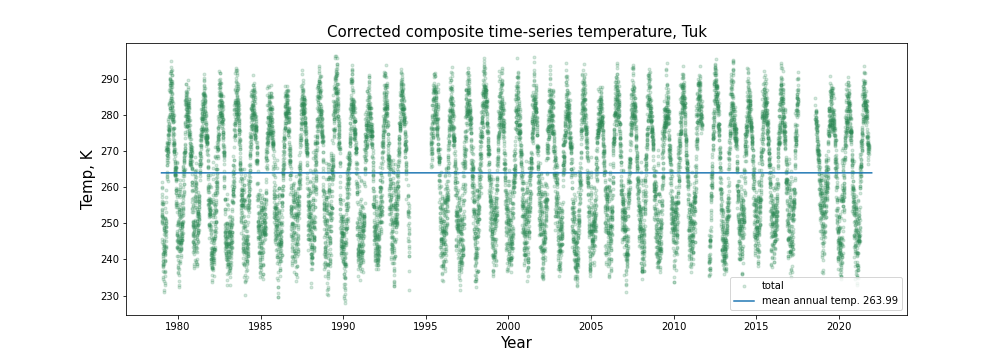
\includegraphics[scale=0.5]{figures/Tuktemp.png} \label{fig:a}} \\
  \subfloat{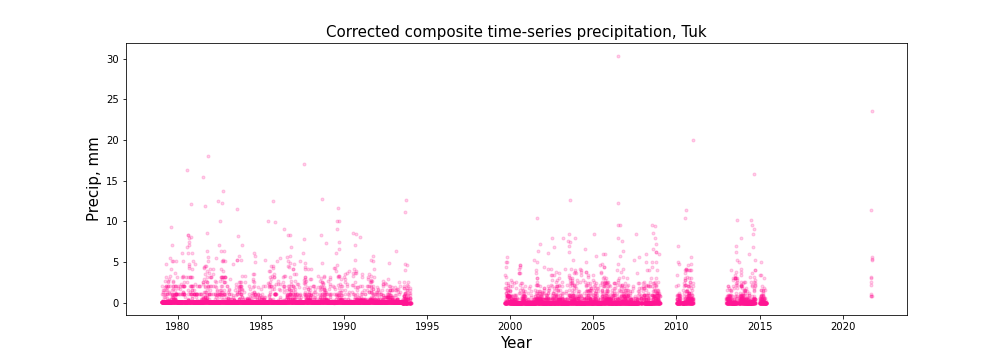
\includegraphics[scale=0.5]{figures/Tukprecip.png} \label{fig:b}} \\
  \subfloat{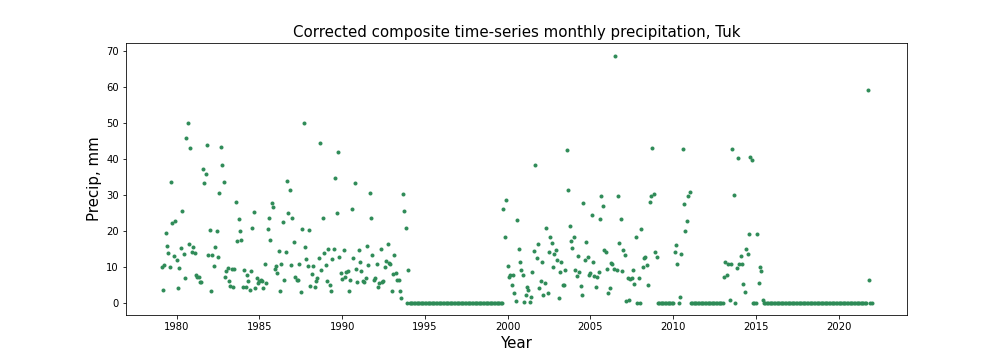
\includegraphics[scale=0.5]{figures/Tukmonthly_precip.png} \label{fig:c}}
  \caption{Plots of temperature (a), precipitation (b) and daily precipitation (c) for Tuktoyaktuk.} \label{fig:AB}
\end{figure}




\begin{figure}
  \centering
  \subfloat{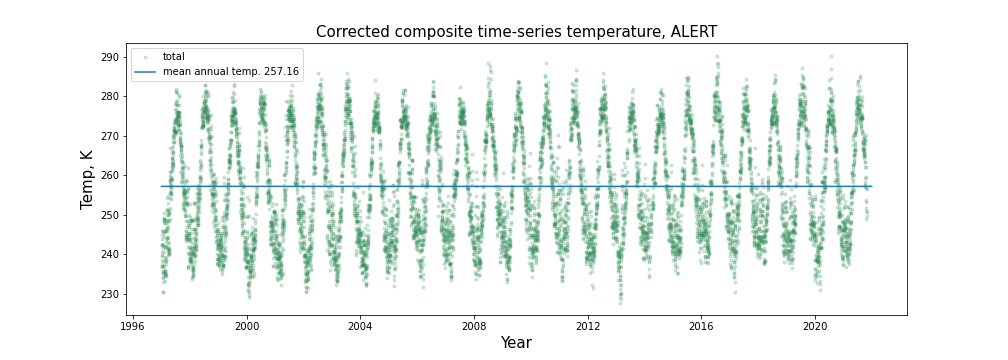
\includegraphics[scale=0.5]{figures/ALERTtemp.png} \label{fig:a2}} \\
  \subfloat{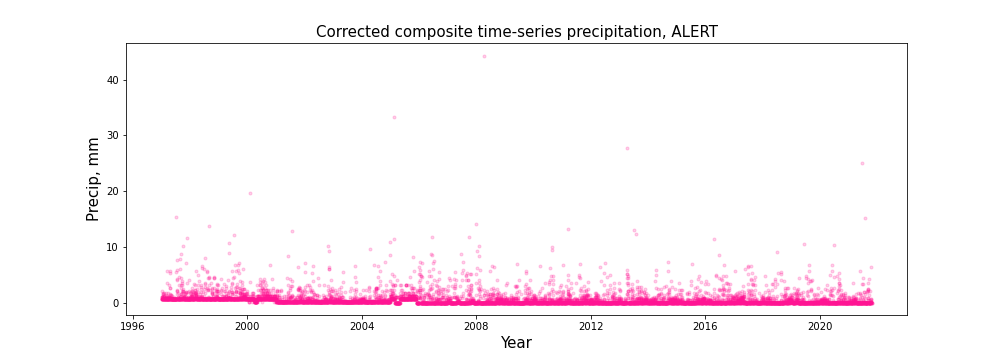
\includegraphics[scale=0.5]{figures/ALERTprecip.png} \label{fig:b2}} \\
  \subfloat{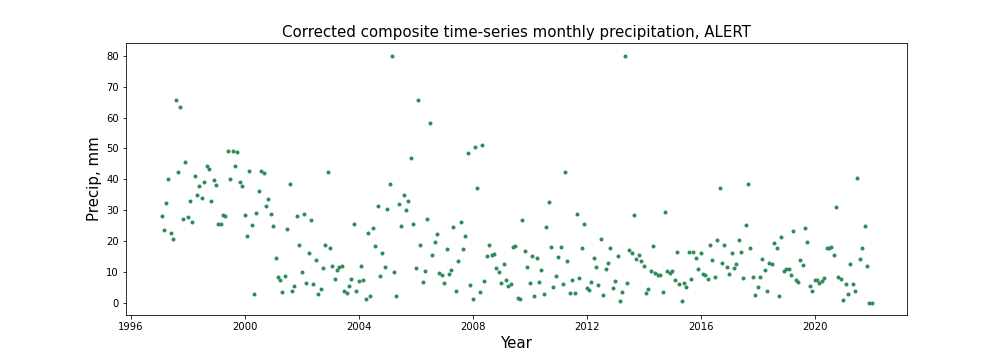
\includegraphics[scale=0.5]{figures/ALERTmonthly_precip.png} \label{fig:c2}}
  \caption{Plots of temperature (a), precipitation (b) and daily precipitation (c) for ALERT.} \label{fig:AB2}
\end{figure}

\begin{figure}
  \centering
  \subfloat{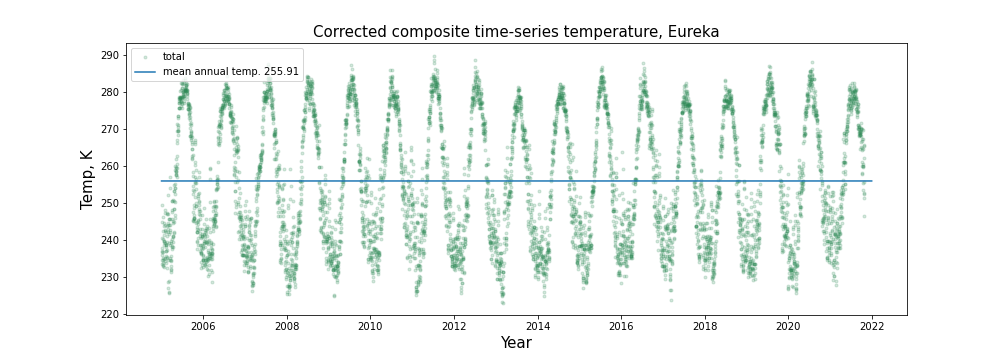
\includegraphics[scale=0.5]{figures/Eurekatemp.png} \label{fig:a3}} \\
  \subfloat{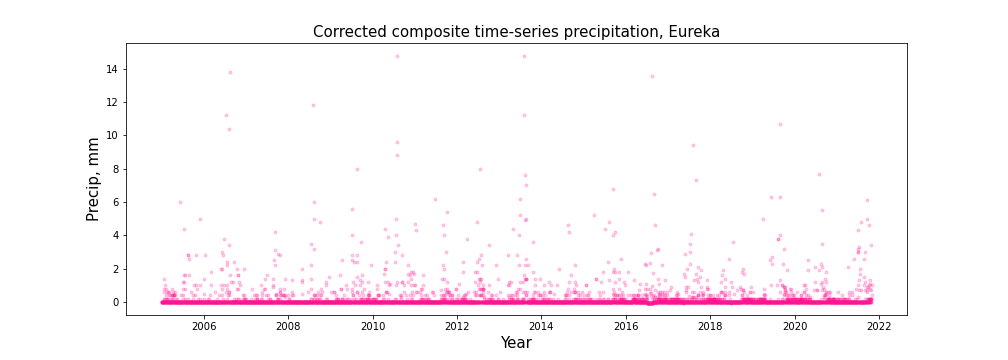
\includegraphics[scale=0.5]{figures/Eurekaprecip.png} \label{fig:b3}} \\
  \subfloat{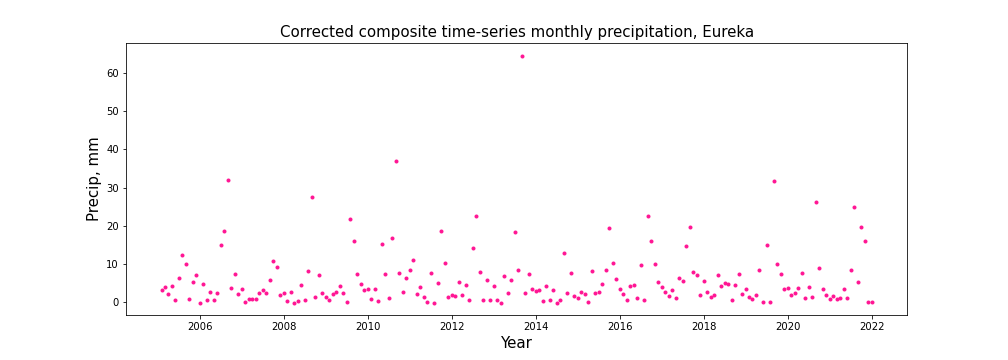
\includegraphics[scale=0.5]{figures/Eurekamonthly_precip.png} \label{fig:c3}}
  \caption{Plots of temperature (a), precipitation (b) and daily precipitation (c) for Eureka.} \label{fig:AB3}
\end{figure}



%The heatmaps are shown in figures \ref{eurekap_47_21}, \ref{eurekap_16_21}, \ref{eurekah_47_21} \& \ref{eurekah_16_21}. 

\begin{comment}
?? include all plots here once I have decided what to do with them 



\begin{figure}[hbtp]
\centering
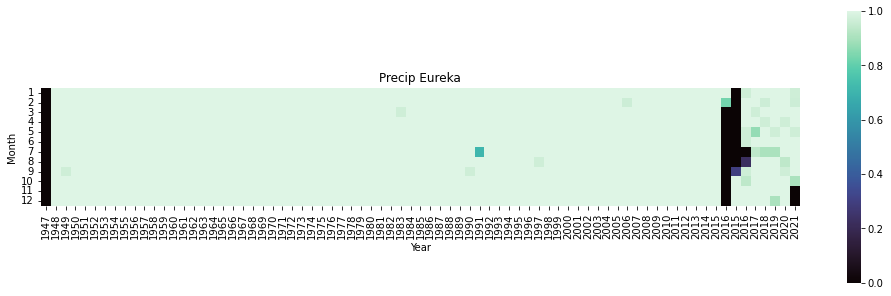
\includegraphics[width=0.99\textwidth]{figures/eureka_precip_1947_2021.png}
\caption{Heatmap of data availability for daily precipitation at Eureka from 1947 to 2021. Each month is represented by a square, with a full month of data in green and no data in black.  }\label{eurekap_47_21}
\end{figure}

\begin{figure}[hbtp]
\centering
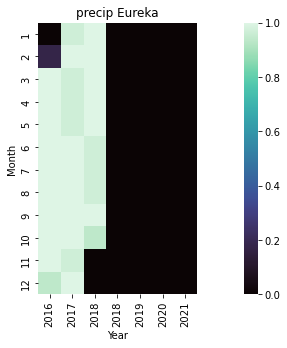
\includegraphics[width=0.2\textwidth]{figures/eureka_precip_2016_2021.png}
\caption{Heatmap of data availability for daily precipitation at Eureka from 2016 to 2021. Each month is represented by a square, with a full month of data in green and no data in black.  }\label{eurekap_16_21}
\end{figure}

\begin{figure}[hbtp]
\centering
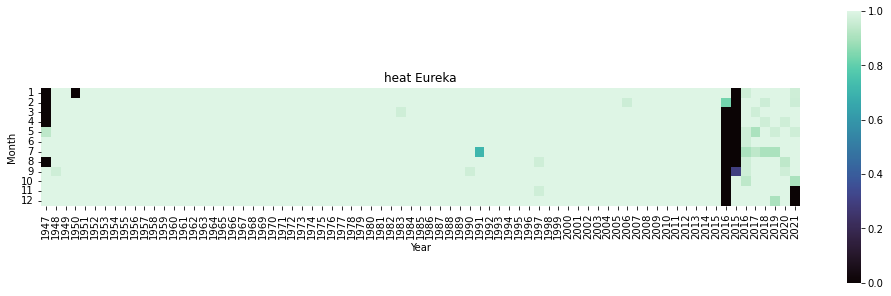
\includegraphics[width=0.99\textwidth]{figures/eureka_temperature_1947_2021.png}
\caption{Heatmap of data availability for daily mean temperature at Eureka from 1947 to 2021. Each month is represented by a square, with a full month of data in green and no data in black.  }\label{eurekah_47_21}
\end{figure}

\begin{figure}[hbtp]
\centering
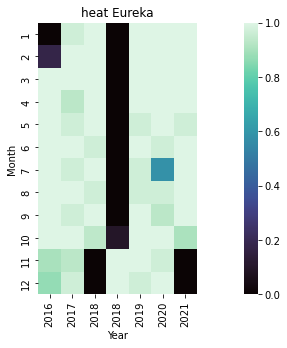
\includegraphics[width=0.2\textwidth]{figures/eureka_temperature_2016_2021.png}
\caption{Heatmap of data availability for daily mean temperature at Eureka from 1947 to 2021. Each month is represented by a square, with a full month of data in green and no data in black.  }\label{eurekah_16_21}
\end{figure}

\end{comment}



\begin{comment}
\subsubsection{Analysing duplicates}
For many stations there were more than two readings for each day. To see if these were duplicates or different measurements taken with different instruments, for months where there was repetition, plots were produced comparing the data. 
\paragraph{Eureka}
For Eureka, there were only duplicates for 2016 onwards.

There were minor differences in temperature and precipitation readings for these times.



\begin{figure}[!tbp]
  \centering
  \begin{minipage}[b]{0.99\textwidth}
    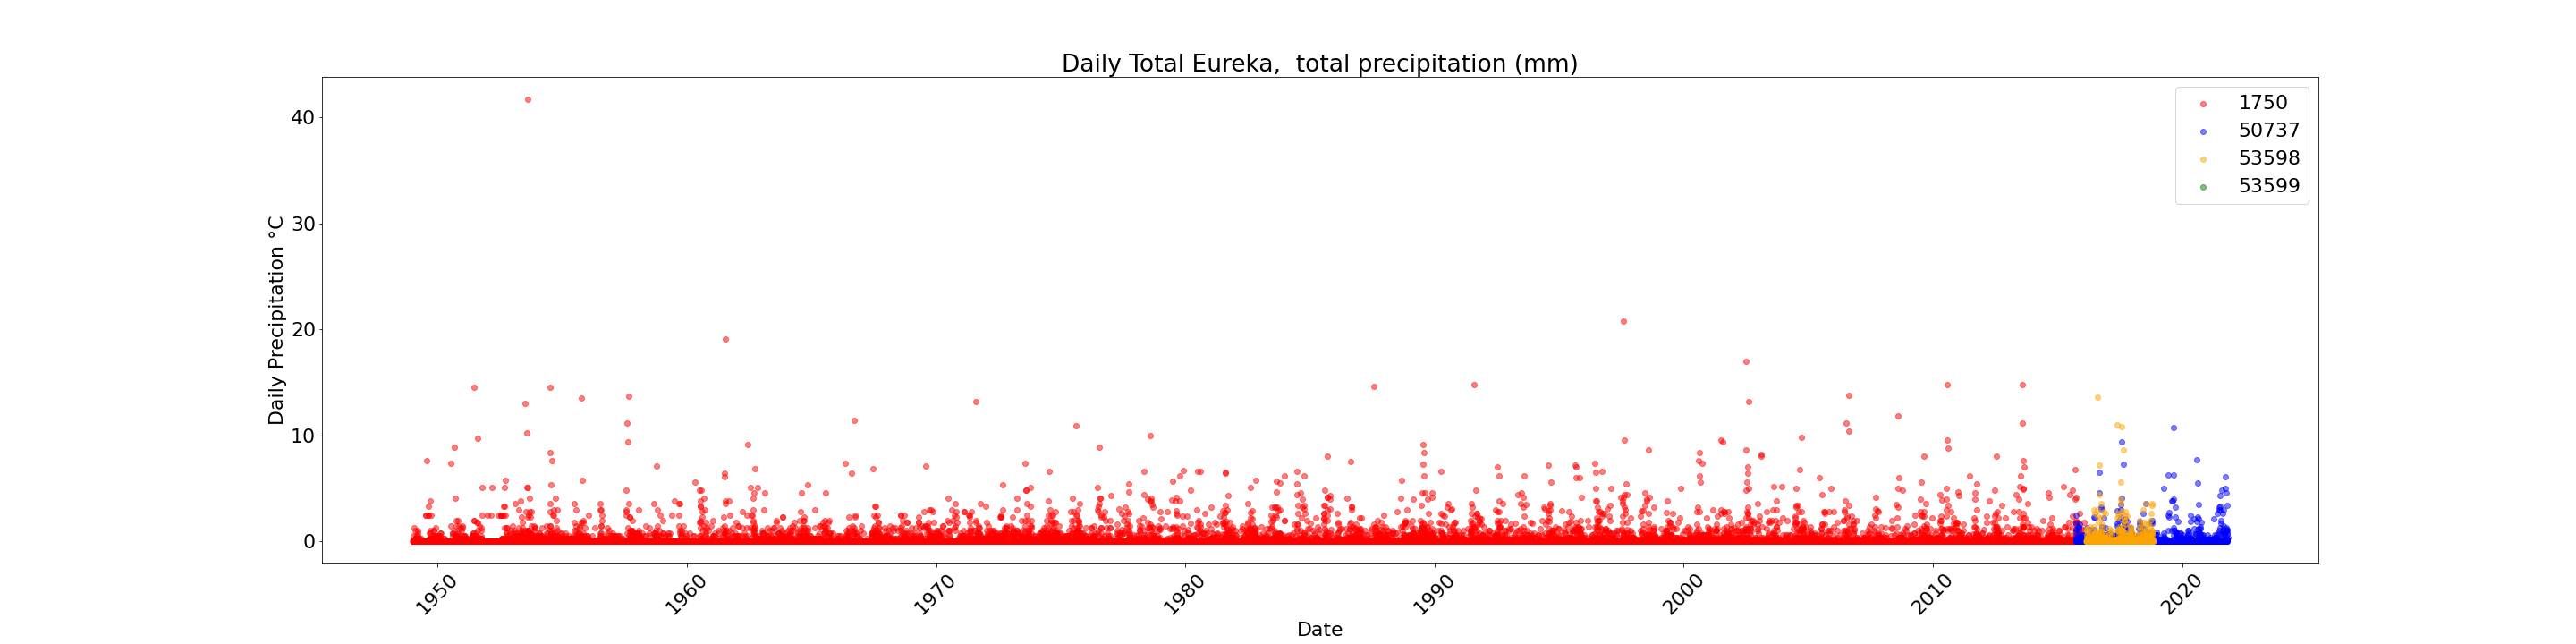
\includegraphics[width=\textwidth]{figures/daily_totalEureka, totalprecipitation(mm).png}
  \end{minipage}
  \begin{minipage}[b]{0.99\textwidth}
    \includegraphics[width=\textwidth]{figures/daily_totalEureka, mean temperature °C.png}
  \end{minipage}
  \caption{Daily mean temperature measurements and total precipitation  for Eureka from 1949 to present day. }\label{fig:yearly_eureka}
\end{figure}



\paragraph{Alert}
For Alert, there were only duplicates for 1997 onwards.

There were minor differences in temperature and precipitation readings for these times.


readings for these times.


\begin{figure}[!tbp]
  \centering
  \begin{minipage}[b]{0.99\textwidth}
    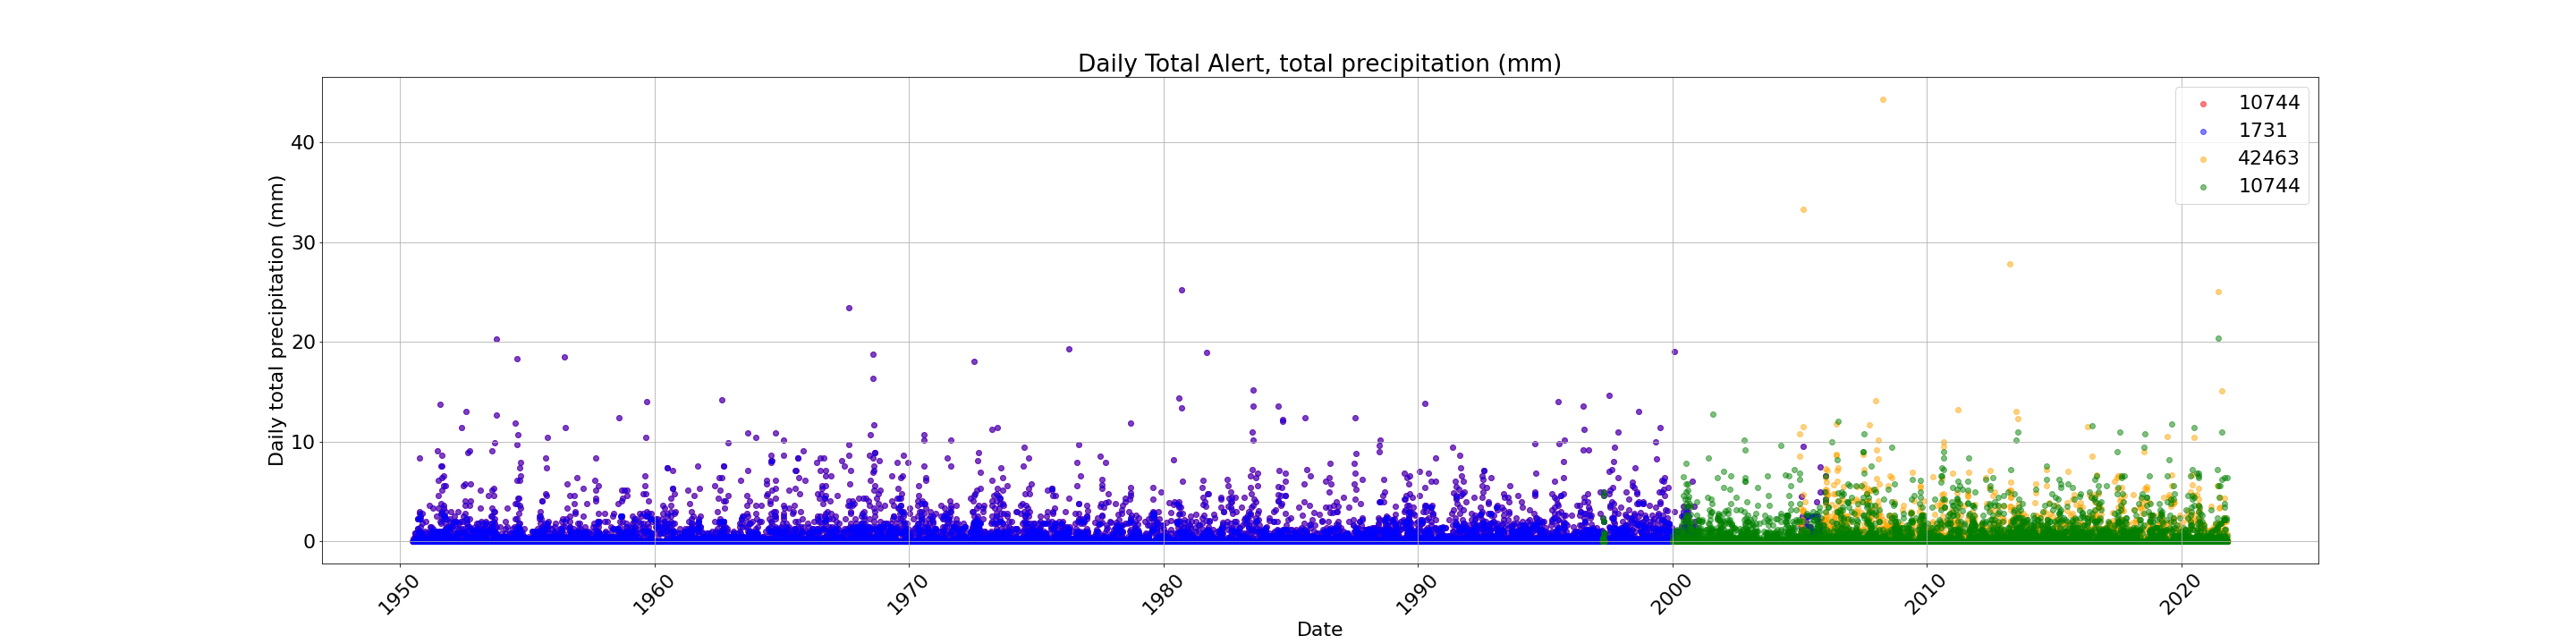
\includegraphics[width=\textwidth]{figures/daily_totalAlert, total precipitation (mm).png}
  \end{minipage}
  \begin{minipage}[b]{0.99\textwidth}
    \includegraphics[width=\textwidth]{figures/daily_totalAlert, mean temperature °C.png}
  \end{minipage}
  \caption{Daily mean temperature and total precipitation measurements for Alert from 1950 to present day. }\label{fig:yearly_alert}
\end{figure}


\paragraph{Tutoyaktuk}
For Tutoyaktuk, there were only duplicates for 1979 onwards.

There were minor differences in temperature and precipitation readings for these times.


\begin{figure}[!tbp]
  \centering
  \begin{minipage}[b]{0.99\textwidth}
    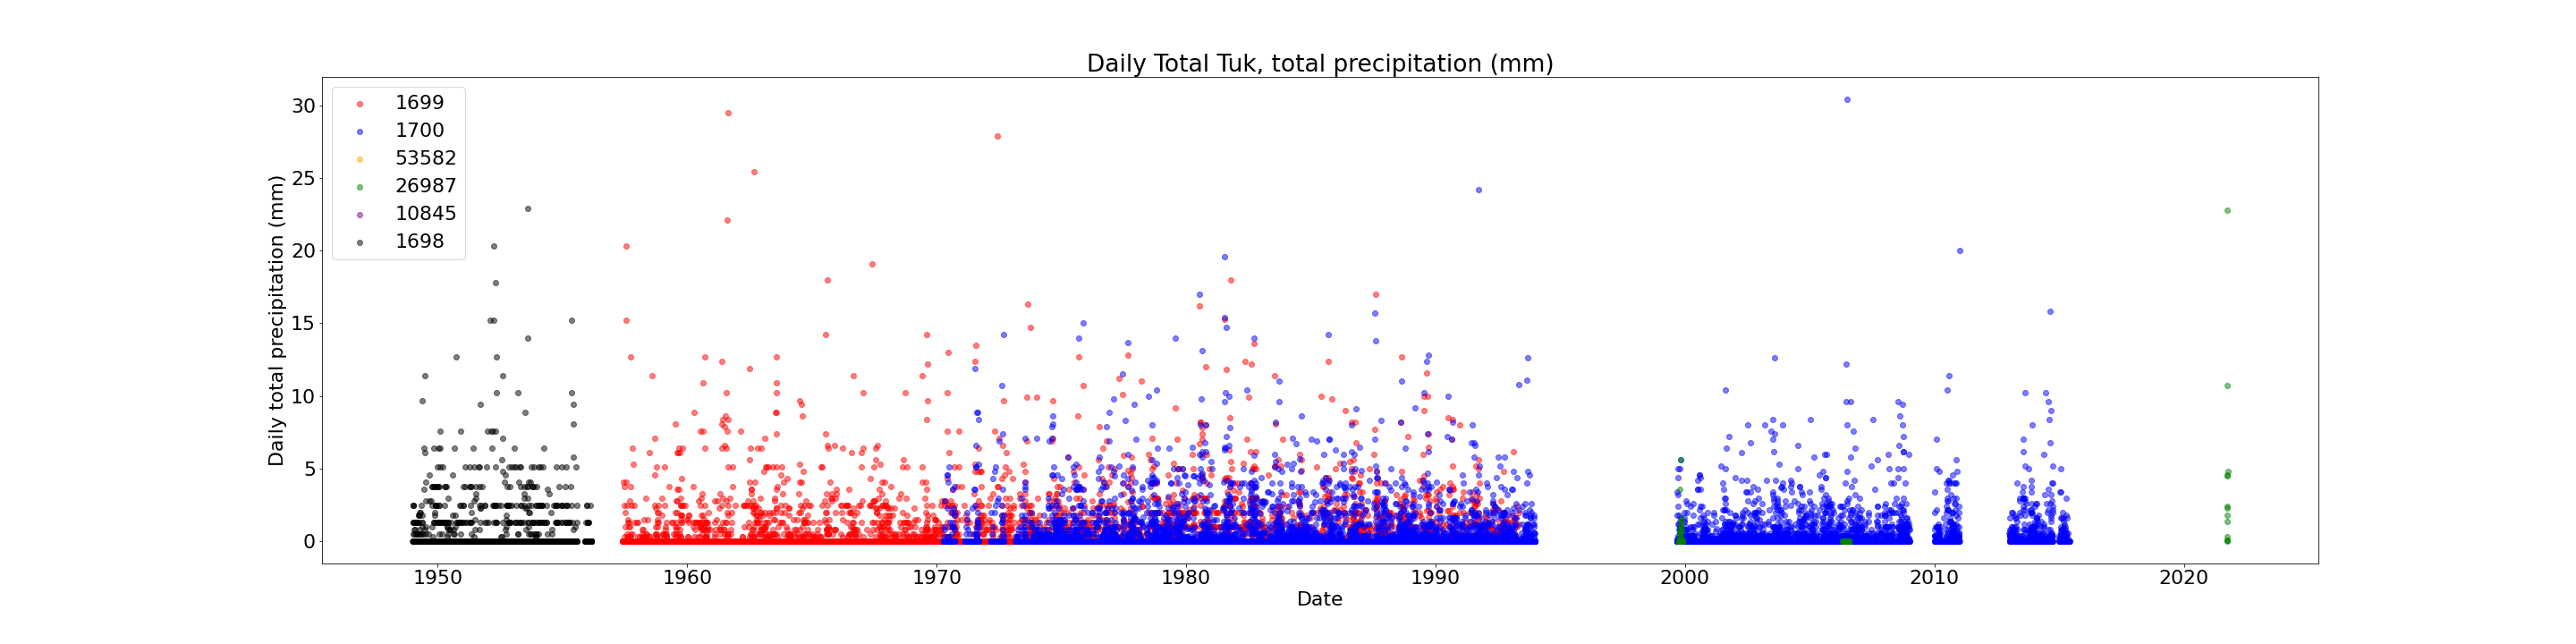
\includegraphics[width=\textwidth]{figures/daily_totalTuk, total precipitation (mm).png}
  \end{minipage}
  \begin{minipage}[b]{0.99\textwidth}
    \includegraphics[width=\textwidth]{figures/daily_totalTuk, mean temperature °C.png}
  \end{minipage}
  \caption{Daily mean temperature and total precipitation measurements for Alert from 1949 to present day.}\label{fig:yearly_tuk}
\end{figure}

\end{comment}


\subsection{Reanalysis methods}


{\color{blue}- What is reanalysis and what is its function
- How do I compare the reanalysis to the historical measurements?
}

Due to temporal and spatial biases, complete weather measurements for the past are not available, as seen in the plots from section 
\ref{section:historical}. Measurements from the past which are available are not evenly distributed around the globe, particularly for areas in harsh environments with small populations

Reanalysis products combine measurements from the past with up to date weather models to create a full picture of what the weather was like in the past. These data sets provide comprehensive weather and climate conditions at regular intervals overtime and are used in atmospheric dynamics, climate stability and for evaluating climate models. In this study reanalysis models are used in replacement of historical measurements since raw data is sparce for areas in the WCA. 

Reanalysis models have errors associated with them and often have biases due to changing observation methods. This aside, they are useful and critical to researching climate in the recent past. 


\subsubsection{Reanalysis validation}
There are a number of different reanalysis datasets available for study in the Arctic. The ERA-5 dataset was chosen as it since it has data available from 1979 to present day, with the
highest correlation coefficients compared with experimental weather data, small biases and
root mean square errors, compared with other reanalysis datasets \cite{era5,era5veari}. 
%\cite{era5veari}

To verify that the reanalysis data sets were suitable for use in this project, reanalysis measurements for precipitation and temperature were compared with experimental measurements from section \ref{section:historical}. Janurary 2008 was chosen since there was a weather event during this period, characterised by the increases in temperature at all three stations. The plots below comparing temperature for the three stations show considerable agreement, signifying that the original measurements were assimilated, or use in creating the reanalysis product. 


\begin{figure}[h!]
  \centering
  \subfloat{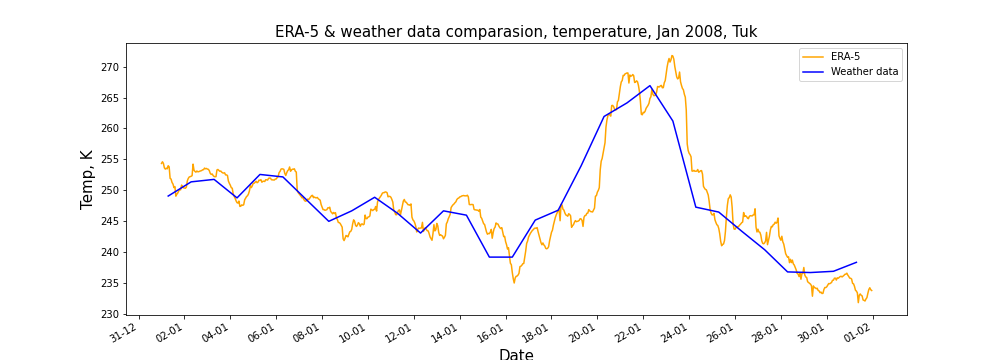
\includegraphics[scale=0.5]{figures/Tuktemp_era5.png} \label{fig:tuk}} \\
  \subfloat{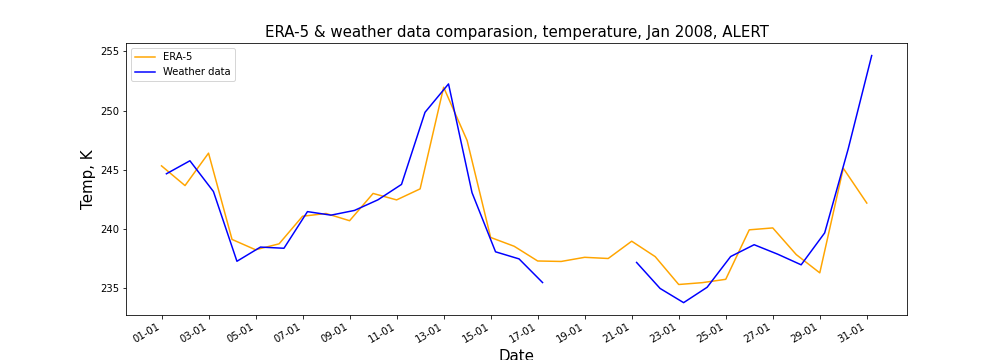
\includegraphics[scale=0.5]{figures/ALERTtemp_era5.png} \label{fig:alert}} \\
  \subfloat{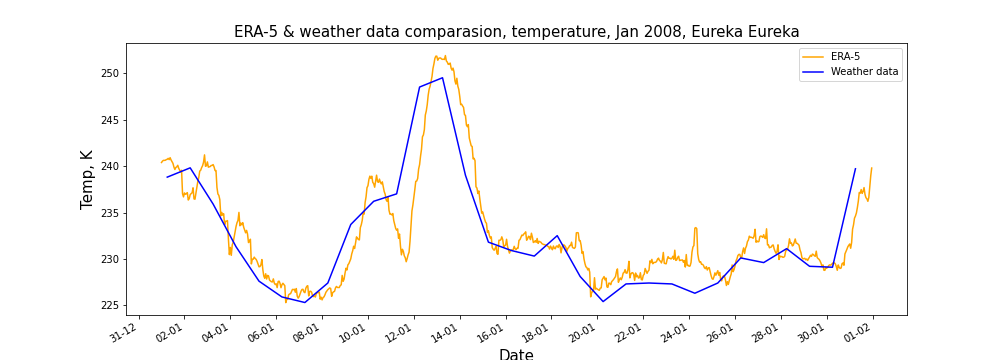
\includegraphics[scale=0.5]{figures/Eurekatemp_era5.png} \label{fig:erueka}}
  \caption{Plots of Tuktoyaktuk (a), ALERT (b) and Eureka (c) comparing temperature measurements for January 2008.} \label{fig:AB4}
\end{figure}

Since these measurements show such good agreement it was verified that the ERA-5 dataset was suitable for use in this project. 

\newpage

\subsection{Hysplit}
%Plotting the ERA-5 datasets in Panoply, allows for identification of weather events and un
Hysplit is an atmospheric dispersion modelling software used for computing air parcel trajectories, and in this study is used to determine the origin of air masses. 

Hysplit is used to establish where the changes in moisture are coming from. Using wind measurements from ERA-5 Hysplit is used to track the origins of events with high humidity. 
\newpage 


%\bibliographystyle{alpha}
 \bibliography{references}{}
\bibliographystyle{apalike}




\end{document}